\chapter{More projects}
\thispagestyle{fancy}
\label{ch:more-projects}


\project{Reisdorf river dam}
\label{pr:reisdorf}
To obtain a reliable source of drinking water and energy, the river S\^{u}re was dammed near Esch-sur-S\^{u}re during the 1960s. The resulting Lake of the Upper S\^{u}re is now one of the most popular vacation spots in Luxembourg. The successful exploitation of this artificial lake has persuaded the city council of Reisdorf to construct a dam of their own. They expect that the fresh water, energy and flourishing tourist industry will bring them health and wealth. The city council has asked a team of experts from the University of Amsterdam to research the consequences of the erection of such a dam. In this exercise, we will simulate the flooding of the Ernz Blanche river valley.
\begin{action}
Set your work directory to the folder `\textbackslash{}ch12\_more\_projects\textbackslash{}proj06\_reisdorf'. 
\end{action}
\begin{action}
Load the files into the workspace using:
\end{action}
\lstinputlisting[numbers=none,nolol]{./../m/load_ebd.m}
\begin{action}
Visualize the Ernz Blanche DEM. 
\end{action}
\begin{action}
The file `dam\_height.txt' contains data on the dimensions and location of the dam. Visualize the dam by using {\tt imagesc}, then use the zoom-in feature to inspect the top rows where the Ernz Blanche leaves the map. The correct surface elevation data -after construction of the dam- is obtained by adding the values in {\tt DamHeight} to {\tt EBD}.  
\end{action}
To analyze the consequences of the dam, you need to have insight in the water input into the system. Based on historical data, we have a dataset (`ebsupply.txt') with the volumes of water [m$^{3}$] that will flow into the lake each month once the dam is closed. 
\begin{action}
Visualize the data from `ebsupply.txt'.
\end{action}
The first 3 years after construction, the dam is kept closed to allow the water level to rise behind the dam for a profitable dam discharge.
\begin{action}
Calculate the volume of water that has accumulated behind the dam in these 3 years.
\end{action}
We would like to know which area is flooded after these three years.
\begin{action}
Why is it not possible to calculate the water level directly from the water volume?
\end{action}
In contrast to the difficulty in calculating the water level from the water volume, the reverse problem is quite easy: suppose you would know the water level {\tt h}, the grid cell dimensions and the grid cell elevation (the DEM), it would be relatively easy to calculate the water volume beneath this water level. In this exercise, we will exploit this to approximate the true water level. A function has already been created that calculates water volume under a given water height, but accidentally it was messed up. The command lines are intact, but the order is wrong. The code can be found in the file `mess.txt'.
\begin{action}
Put the lines in `mess.txt' in the right order and save the file as `\starred{name}\_calcvol.m' (with your last name for \starred{name}). Refer to Chapter~\ref{ch:functions} if you forgot how a function is structured.
\end{action}
\hintbox{Variables that occur after the `='-sign must have been assigned previously; new variables can only occur before the `='-sign.}
\begin{action}
To test if you changed the order of the lines correctly, type
\prompt{sum(sum(calcvol(241.1318,EBD+DamHeight,25,25)))}
(don't forget to add your last name to the function call). This should return 1.0000e+007.
\end{action}
\begin{action}
If {\tt h}, {\tt CellSizeX} and {\tt CellSizeY} are in meters, what are the units of this result?
\end{action}
To be able to assess which grid cells of the DEM are flooded by the water in the lake after three years, you need to calculate the water level (above sea level) given the calculated water volume. Since it is not possible to calculate {\tt h} directly, you must use an approximation method. This approximation method is used to try out a number of assumed water levels. For each assumed water level, you can calculate the water volume that is associated with it using {\tt calcvol}. The water volume that is associated with the assumed water level is then compared to the actual water volume of the lake (which we can get from the values in {\tt EBSupply}). If the assumed volume is too low, we need to adjust the assumed water level upward; if the assumed water volume is too high, we need to adjust the assumed water level downward. With each adjustment, the interval containing the true water level decreases. We need to keep adjusting until the interval has become sufficiently small. An efficient way for adjusting the value of water level is the so-called 'bisection method'\index{bisection method}. The first step of the bisection method is to define the \textul{initial} lower {\tt hLo} and upper {\tt hUp} bounds on the water level. At any point during the approximation, the interval [{\tt hLo},{\tt hUp}] is as small as possible, given the knowledge that has been collected so far about the true water level {\tt hAct}.
\begin{action}
Determine the lowest (bottom of the lake) and highest (maximum height in the DEM) water levels. These values form the initial estimates of {\tt hLo} and {\tt hUp} (\textit{Step 1}, see Figure~\ref{fig:water-levels}).
\end{action}
\begin{action}
{\tt hMid} is defined as the average of {\tt hLo} and {\tt hUp}. Calculate the corresponding water volume with {\tt calcvol} (\textit{Step 2}, see Figure~\ref{fig:water-levels}).
\end{action}

\noindent The actual water volume is either between the volume associated with {\tt hLo} and {\tt hMid}, or between {\tt hMid} and {\tt hUp}, meaning that the actual water level is also in that interval. Since you now know whether the actual water level {\tt hAct} is in the lower part or the upper part, you eliminate the part that does not contain {\tt hAct} by redefining either {\tt hLo} or {\tt hUp} (\textit{Step 3}, see Figure~\ref{fig:water-levels}).

\noindent In Step 3 of the figure, {\tt hLo} remains unchanged with respect to its position in Step 2, whereas the former {\tt hMid} (see Step 2) is now defined as {\tt hUp}, since you found out that the actual {\tt hAct} is certainly not in the Step 2-interval [{\tt hMid},{\tt hUp}]. Steps 2 and 3 are repeated until the interval [{\tt hLo},{\tt hUp}] has become small enough to meet your preset criterion.

\begin{action}
Finish Figure~\ref{fig:water-levels} by drawing lines in the lower right subplot. Assign each line a label {\tt hLo}, {\tt hMid}, and {\tt hUp}.
\end{action}

\begin{figure}[htbp]
  \centering
    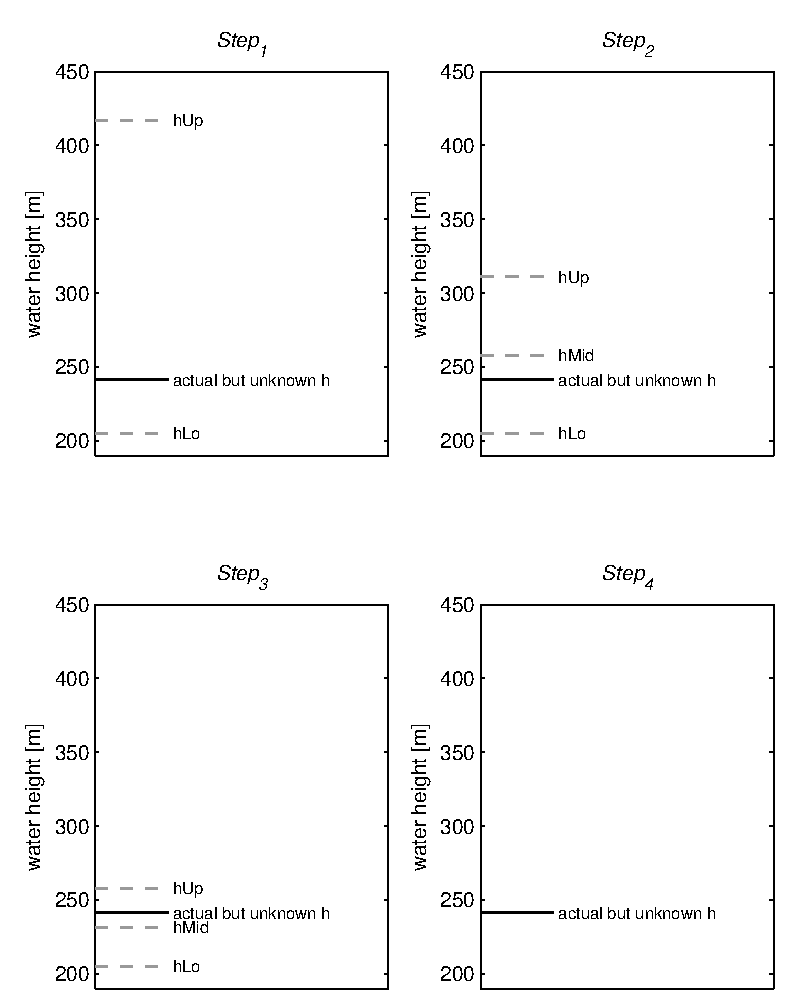
\includegraphics[width=1.0\textwidth]{./../eps/water-levels.eps}
  \caption{Graphical demonstration of the bisection method.}
  \label{fig:water-levels}
\end{figure}


\noindent In the next few exercises, you will implement the bisection technique in a function that can be used to approximate the actual water level associated with a given water volume behind the dam. This function is subsequently used to approximate the water depth of the lake for each month during the first three years after the dam was erected. The function that you will be developing uses the function {\tt calcvol} that you already made.


\begin{action}
First think of the input variables that you need and the output that you want. Together this determines the function call.
\end{action}
\begin{action}
A rough setup of the program is given in the function m-file `outline.m'. Save this file as `\starred{name}\_approxh.m' (where \starred{name} is your last name) and edit this file until it produces the right result as shown in Figure~\ref{fig:lake-reisdorf-36-months}.
\end{action} 

\begin{figure}[htbp]
  \centering
    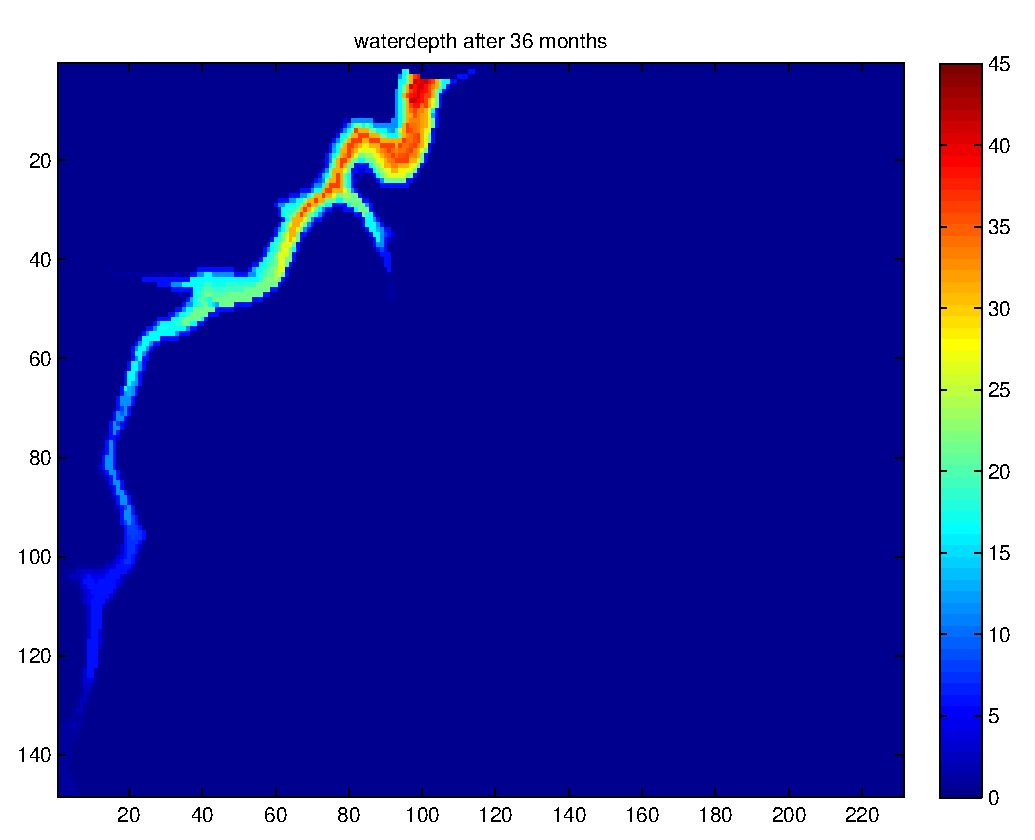
\includegraphics[width=0.75\textwidth]{./../eps/lake-reisdorf-36-months.eps}
  \caption{Distribution of water depths 36 months after the dam was closed.}
  \label{fig:lake-reisdorf-36-months}
\end{figure}

\noindent We are not only interested in the inundated area after three years, but we would like to know the inundated area for each month after the closure of the dam and as long as the water level has not reached the upper level of the dam.

\begin{action}
Start a new script called `\starred{name}\_reisdorf.m' (with your last name for \starred{name}). Let your script visualize the water depth in the valley for each month after the closure of the dam, starting from the dry situation and continuing until the valley is filled up to the upper level of the dam. Use the {\tt approxh} function and the {\tt calcvol} function that you have already written.
\end{action}

\noindent So far, we have used {\tt imagesc} in its simplest form: {\tt imagesc(X)}. This form visualizes the array {\tt X} using a gradient of colors. The colors are automatically set in such a way that they range from the minimium of {\tt X} to the maximum of {\tt X}. However, sometimes you want to set these color limits yourself. For this, you can use {\tt imagesc} with a second input argument: {\tt imagesc(X,C)}\index{imagesc@\texttt{imagesc}}, where {\tt C} is a 1x2 numeric variable, with the user-specified color limits. For instance, in the Reisdorf example of Figure~\ref{fig:lake-reisdorf-36-months}, the minimum color has been set to 0, whereas the maximum color has been set to 45. The command to do this is: {\tt imagesc(WaterDepth2D,[0,45])}.

\begin{action}
Use the 2-argument form of {\tt imagesc} to set the color limits on your water depth figure.
\end{action}

\section{Making movies}
\index{movie}
Extensive calculation results often ask for some kind of animated output. For example, the filling of the reservoir could be visualized as a function of time. In this section you learn how you can save these animations\index{animation} in movies that can be shown without having to run the \MATLAB{} program again.

\noindent A movie consists of frames\index{frame}, just like a traditional celluloid movie. You need to initialize the movie by including the following line in the initialization part:
\begin{lstlisting}[numbers=none]
aviObj = avifile('testmovie.avi','fps',5,...
                         'compression','none');
\end{lstlisting}\index{avifile@\texttt{avifile}}

\noindent This example initializes a movie file `testmovie.avi'. Using the {\tt \squote{fps}}\index{`fps@\texttt{\squote{fps}}} (for `frames per second') option, you can specify at what speed you want to play the movie later. In the example, a frame rate\index{frame rate} of 5 frames per second\index{frames per second} is used. Furthermore, you can specify the compression algorithm that \MATLAB{} will use. For now, we will set {\tt \squote{compression}}\index{`compression@\texttt{\squote{compression}}} to {\tt \squote{none}}, but we will return to this later in Section~\ref{ch:compression}. Running the above command will create a variable {\tt aviObj} of data class `avifile object'. (You can check this in the workspace). See {\tt doc avifile} for more details.

\noindent After the avifile object has been initialized, you can add as many frames as you like (as long as there is available space on your harddisk). After issuing the visualization commands (such as {\tt imagesc}, {\tt scatter}, {\tt surf} or {\tt plot}), you need to capture\index{capture} the frame and add it to your avifile object variable. A generic structure of a script that creates a movie is included in \lstlistingname~\ref{list:generic-moviecapture}.
\lstinputlisting[float,label={list:generic-moviecapture},caption={Generic structure of a script that creates an *.avi\index{*.avi file extension} movie.}]{./../m/generic_moviecapture.m}

\subsection{On the need for closure}
It is crucial that your program gets to closing the avifile object. If you forget to include this part, or if the program crashes before it gets to closing the avifile, you end up with an *.avi file (in this case `testmovie.avi') which cannot be played. This is because media players will wait for \MATLAB{} to release its handle on the file (which it never will, since the program crashed). If this is the case, you need to issue a {\tt clear all}\index{clear all@\texttt{clear all}} \textit{at the prompt}. Note that you will generally not include the {\tt clear all} in your script, since it makes debugging impossible. For this course, we will \textit{only} use {\tt clear all} when dealing with movies that have not been finalized. In all other situations, you need to use {\tt clear}.
\begin{action}
Change your program in such a way that it creates a movie of the filling of the artificial lake for each month for the first 3 years. 
\end{action}

\begin{action}
Re-read the part about {\tt for}-loops and {\tt while}-loops on page \pageref{sec:for-loops}--\pageref{sec:while-loops}. Now change your script in such a way that it keeps calculating the monthly water depth map for as long as the water level is lower than the level of the dam.
\end{action}


\subsection{Compression}
\label{ch:compression}
As you may have noticed, making a movie without using any compression can generate big files, especially when you are capturing many frames. This is where compression algorithms come in handy. Compression algorithms, or codecs\footnote{\url{http://en.wikipedia.org/wiki/Codec}}\index{codec}, are used to decrease file size, while maintaining as much of the original quality as possible. In this respect, they are similar to what MP3 is for audio, what JPEG is for photos, or what ZIP is for data. Codecs are well worth looking into, because a good codec can decrease a file by a factor 100 without compromising the movie quality!

\begin{action}
In your work directory, there is a codec file `mpg4c32.dll', which can be used to compress your movie file. In order for this to work, you need to set the {\tt \squote{compression}} option to {\tt \squote{mpg4}}. Make the necessary changes to have your program use this compression algorithm. 
\end{action}



\projectfooter{}



\project{Flow path}
The characteristics of a drainage network play a great part in determining how water moves through a basin and consequently affects issues such as water quality and quantity (including flooding). Drainage patterns dramatically affect people and the environment downstream regardless of administrative borders, often over long distances, and on a very large scale with long-lasting implications. 

In this project, you will analyze water movement in a drainage basin. You will develop a program that calculates the pathway of water for a given DEM, from an arbitrarily chosen starting point to the lowest point of the landscape.
\begin{action}
Set your working folder to `\textbackslash{}ch12\_more\_projects\textbackslash{}proj07\_flowpath', start a new script called `\starred{name}\_flowpath.m' (with your last name for  \starred{name} ) and visualize `valleydem.txt'.
\end{action}
\begin{action}
If you would drop a ball in {\tt valleydem(10,4)}, where would it end up?
\end{action}
To determine water movement in this area, you can use the principle of `steepest descent': this principle is based on the assumption that water movement between cells is driven by the maximum gradient between the origin cell and its 8 surrounding cells.

In order to calculate this maximum gradient, you need to know the difference in height between the origin cell and the surrounding cells ({\tt DeltaH}) and the distance from the surrounding cells to the origin cell ({\tt Dist}). These distances are not all equal.
\begin{action}
Given that the cell dimensions are 25 x 25m, fill the array below with the distances.
\end{action}

\begin{equation}
\mathtt{Dist} = \left[
\begin{array}{ccc}
\ldots&\ldots&\ldots\\
\ldots&0&\ldots\\
\ldots&\ldots&\ldots\\
\end{array}
\right]
\end{equation}
Do you think that you could now write a script to calculate the path water follows from some given starting point to the lowest point? If so, try it. Start with making a design first and then write your program.
If you don't think you can do it just yet, follow the guidelines below.
\begin{action}
What would be the statement to select a 3x3 submatrix {\tt H} from {\tt valleydem} if the position of the center cell in {\tt H} corresponds with {\tt valleydem(68,55)}? If your command is correct, {\tt H} should be equal to:
\end{action}
\begin{verbatim}
 H =
     113.8968  111.6601  109.4644
     115.4084  113.1661  110.9636
     116.9417  114.6987  112.4948
\end{verbatim}
\begin{action}
Create a 3x3 array {\tt DeltaH} with the height differences between the cells and the center cell.
\end{action}
\begin{action}
Create a 3x3 array {\tt Grad} containing the gradients between the origin cell and its neighbors. The gradient is difference in height divided by distance. 
\end{action}
\begin{action}
Set the value of the center cell in {\tt Grad} to 0 to avoid calculation complications with NaN. If you do not want the warning\index{warning@\texttt{warning}} message in your screen, include the following line in your program, just before the line that causes the warning:
\begin{lstlisting}[numbers=none]
warning('off','MATLAB:DivideByZero')
\end{lstlisting}
Remember that divide-by-zero warnings serve a purpose, so make sure you turn them back on after the line that raises the warning. You can do this by:
\begin{lstlisting}[numbers=none]
warning('on','MATLAB:DivideByZero')
\end{lstlisting}
\end{action}
\begin{action}
If one of the gradients in {\tt Grad} is negative, what does that mean?
\end{action}
Now you have a 3x3 array with the values of the gradients of the surrounding 8 cells. The steepest descent-theory states that water flows (only) in the direction of the cell that has the lowest (most negative) gradient. So, the next step is to determine which of the surrounding cells will be the one into which the water flows.
\begin{action}
Create a 3x3 logical array {\tt LocMin} with value 1 on the position where {\tt Grad} has its minimum value.
\end{action}
\begin{action}
Determine the subscripts of the minimum value within {\tt Grad}. Call them {\tt r} and {\tt c}, respectively.
\end{action}
Keep in mind that the location {\tt [r,c]} is the position of the minimum value in {\tt Grad}, not in {\tt valleydem} (see also Figure~\ref{fig:valleydem-grid}).


\begin{figure}[htb]
  \centering
    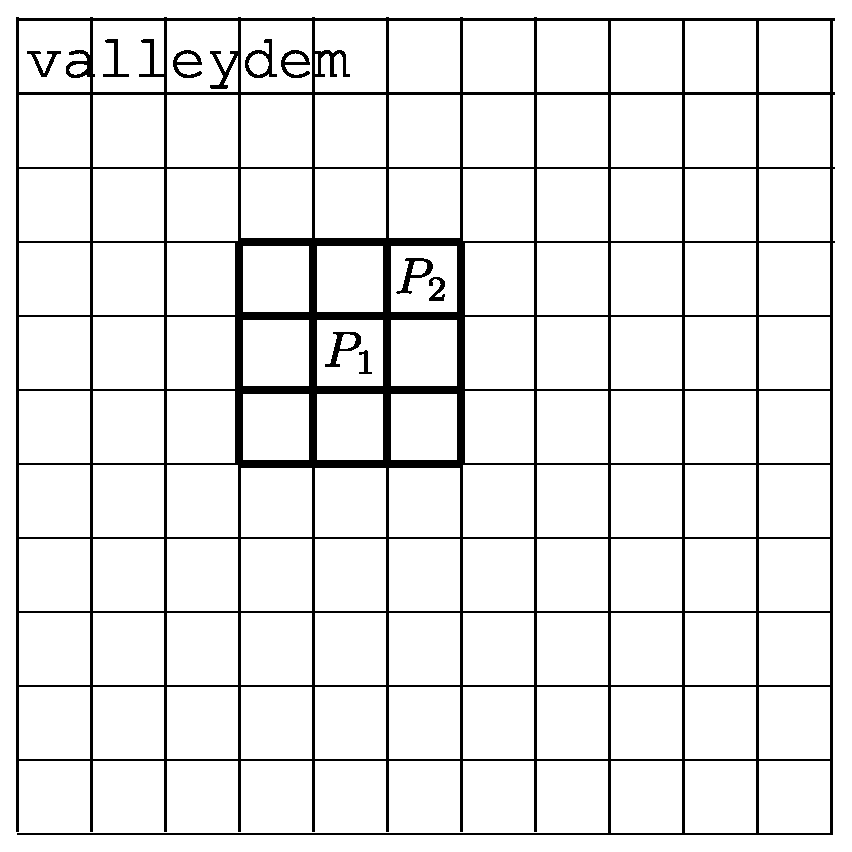
\includegraphics[width=0.5\textwidth]{./../eps/valleydem-grid.eps}
  \caption{The position of {\tt H}, {\tt Dist}, {\tt Grad} within {\tt valleydem}. $P_1$ is the center cell of {\tt H}, {\tt Dist}, and {\tt Grad}, with subscripts r=2 and c=2. The same position in {\tt valleydem} is indicated by ({\tt CurrentRow,CurrentCol}). Position $P_2$ is the position for which the gradient is most negative, i.e., the direction of steepest descent.}
  \label{fig:valleydem-grid}
\end{figure}


\begin{action}
What is the range of valid values for {\tt r}? And for {\tt c}?
\end{action}

\begin{action}
If $P_1$ is the position ({\tt 68},{\tt 55}) in {\tt valleydem}, what is the position of $P_2$?
\end{action}


\begin{action}
If $P_1$ is the position ({\tt CurrentRow},{\tt CurrentCol}) in {\tt valleydem}, what is the position of $P_2$?
\end{action}

\begin{action}
We can use the subscripts of $P_2$ (with respect to {\tt Grad}) to determine its position within {\tt valleydem}. Alter your script in such a way that {\tt CurrentRow} and {\tt CurrentCol} are updated based on the value of {\tt r} and {\tt c}.
\end{action}

\noindent At this point, we have all the necessary constituents for repeating the following steps in a for-loop:
\begin{enumerate}
\item From {\tt valleydem}, select the 3x3 subset around the current location;
\item Calculate the location of lowest gradient;
\item Make the location of lowest gradient the current location.
\end{enumerate}

\begin{action}
Implement the above mentioned steps in your script m-file. Refer to the program outline given in \lstlistingname~\ref{list:flowpath-outline} for guidance on how to structure your program. The result of your program should look like Figure~\ref{fig:flowpath-valleydem1}. Use concatenation commands to keep a record of the value of {\tt CurrentRow} and {\tt CurrentCol}.
\end{action}

\lstinputlisting[float=htbp,caption={Design of a script that calculates the flow path of water through a catchment},label={list:flowpath-outline}]{./../m/outline_project7_flowpath.m}\index{hold on@\texttt{hold on}}\index{hold off@\texttt{hold off}}

\begin{figure}[htbp]
  \centering
    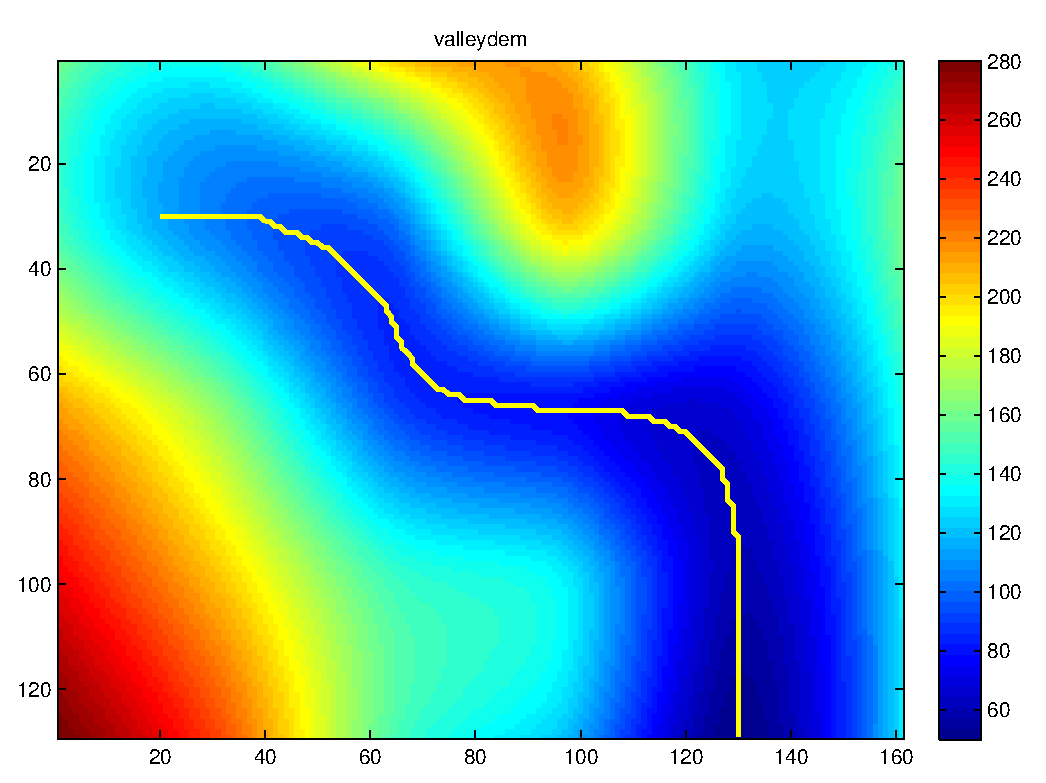
\includegraphics[width=1.0\textwidth]{./../eps/flowpath-valleydem1.eps}
  \caption{Flow path derived from the DEM using the steepest-descent method. Starting point is {\tt valleydem(30,20)}.}
  \label{fig:flowpath-valleydem1}
\end{figure}



\begin{action}
Is it possible to start calculations at position (1,1) of {\tt valleydem}? Why (not)?
\end{action}
At this point, the script m-file calculates the new row and column for 25 iteration steps (see \lstlistingname~\ref{list:flowpath-outline}). However, it is unrealistic that water will stop flowing after 25 steps. What you actually want, is continuous calculation until the borders of the system are reached. 

As opposed to the {\tt for}-loop that performs calculations for a preset number of repetitions, a {\tt while}-loop allows you to perform calculations as long as a certain condition is true. For instance, you could set up a {\tt while}-loop that runs as long as it is {\tt true} that the current position is not on the edge of the domain.

\begin{action}
For which value(s) of {\tt CurrentRow} and {\tt CurrentCol} in {\tt valleydem} can you apply your algorithm? Complete Table~\ref{tab:valleydem-edge}.
\end{action}
\begin{table}[ht]
\caption{While loop conditions}
\label{tab:valleydem-edge}
\centering
\begin{tabular}{|l|p{6cm}|}
\hline
\textbf{Condition}&\textbf{Relational expression in \MATLAB{}}\\
\hline
{\tt CurrentRow} is greater than 1&\ldots\\
\hline
\ldots&\ldots\\
\hline
\ldots&\ldots\\
\hline
\ldots&\ldots\\
\hline
\end{tabular}
\end{table}



\begin{action}
In your script m-file, replace the {\tt for}-loop with a {\tt while}-loop that combines the conditions as stated above.
\end{action}
\begin{action}
Load `valleydem2.txt' and visualize it. Can you see the difference between {\tt valleydem} and {\tt valleydem2}?
\end{action}
\begin{action}
Try to use {\tt valleydem2} in your drainage program (if needed you can stop your program by simultaneously pressing the `Ctrl' and `c' buttons while clicking in the \MATLAB{} command window. 
\end{action}
As you probably found out for yourself, you end up with a never-ending loop because the new DEM contains so-called pits: local minimums. The track ends in a cell with only higher cells surrounding it. You can overcome this by adding an extra condition in your while-statement that tests if the current position is in a pit or not.
\begin{action}
Alter the expression in your while loop in such a way that it tests for pits.
\end{action}
\projectfooter

\pagebreak


\project{Drainage pattern}
\begin{action}
Copy your script m-file from the previous project to the directory '\textbackslash{}chap12\_more\_projects\textbackslash{}proj07\_drainpattern'  and reset your work folder accordingly. Change the script m-file into a function m-file `\starred{name}\_draintrack.m' (with your last name for \starred{name}), with {\tt StartRow}, {\tt StartCol} and {\tt DEM} as input arguments and {\tt Track} as output:
\end{action}
%\vspace{0.5em}
\begin{lstlisting}[numbers=none]
function Track = draintrack(DEM,StartRow,StartCol)
\end{lstlisting}
To get an impression of the total drainage pattern of this valley system, you must run the algorithm for every possible position in {\tt valleydem}. In order to do this, follow the outline below:
\begin{enumerate}
\item Write a script m-file (`\starred{name}\_drainpattern.m'), with a double {\tt for}-loop that calls {\tt draintrack}. 
\item In your {\tt for}-loop, take increments of 10 to avoid long calculation times. 
\item Most of the initial part and the visualization is now not needed in the function and can thus be transported to the main program. Cut and paste as much as possible from the {\tt draintrack} function to the main program. 
\item Check whether the program works well. Use the debugger if necessary.
\end{enumerate}
\begin{action}
Now also try to use the Luxembourg DEM (`demlux.txt') instead of {\tt valleydem}.
\end{action}
As you can see from the error, an analytical error still exists in our program: during calculation, some operations can not be executed because of incorrect variable dimensions. This happens when the program has to deal with more than one lowest gradient and doesn't know which one to use. A relatively easy way to solve this is by always taking the first point.
\begin{action}
Alter your program to always use the first point, even when there are multiple directions with the same lowest gradient. The end result should look like Figure~\ref{fig:drainpattern}.
\end{action}
\begin{action}
The function m-file `randchoosefrom.m' that is present in your directory, lets you pick a value at random if there is more than one direction of steepest descent. Open the function, read the help block, and incorporate it in your script. Note that it's easy to make an analytical mistake here, which will cause your program to calculate an incorrect result (even though it won't raise an error). So think first about what you need to do, before you start implementing.
\end{action}

%\begin{action}
%Can you explain the fact that some drainage directions are crossing each other?
%\end{action}

\begin{action}
Drainage tracks are shorter when the terrain is relatively flat. Why?
\end{action}



\begin{figure}[htbp]
  \centering
    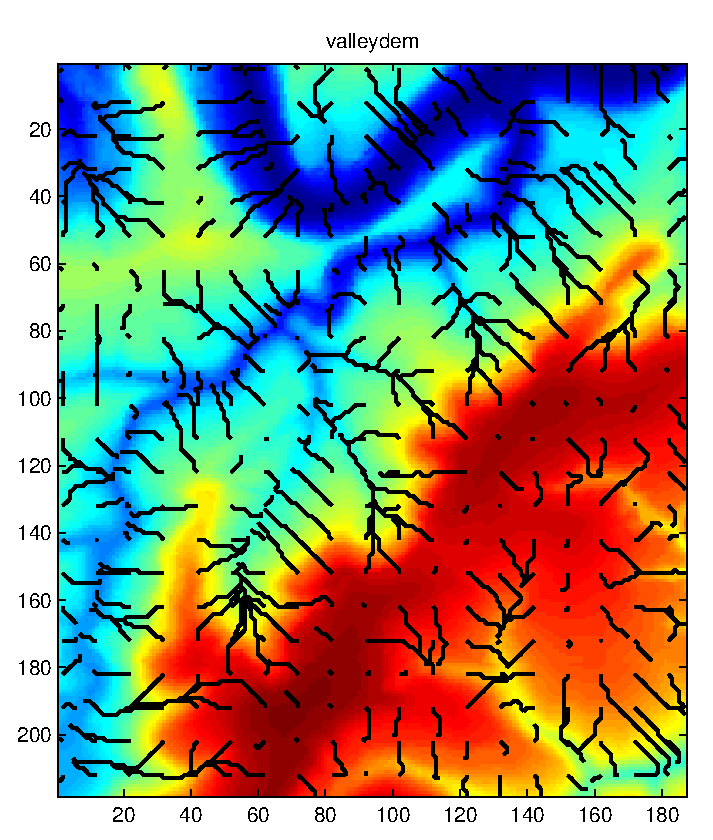
\includegraphics[width=0.75\textwidth]{./../eps/drainpattern.eps}
  \caption{Drainage pattern of the Luxembourg DEM, as determined by the steepest-descent method.}
  \label{fig:drainpattern}
\end{figure}

